\documentclass[presentation]{beamer}
\usetheme{CGA}
\input{package-list-beamer}

%\setbeamercovered{transparent} 

% TODO: Check and remove unneeded figures

\title[Thesis defence presentation]{Characterising antibody immunity and ageing in a short-lived teleost}
\author[William John Bradshaw]{William John Bradshaw}
%\institute[2018 DV Lab Retreat]{Doctoral defence } % TODO: Tinker with this
\date{6th June 2019}

\def\arraystretch{1.2}
\newlength{\slideheight}
\setlength{\slideheight}{0.8\textheight}

\newcommand{\Blackslide}{\blackslide}%\addtocounter{framenumber}{-1}}

\begin{document}

\begin{frame}
\titlepage
\end{frame}

\section{Introduction}

% Slide 1: Title slide

\begin{frame}
% Slide 2: Intro to adaptive immunity
% ~ 1 minute
\begin{figure}
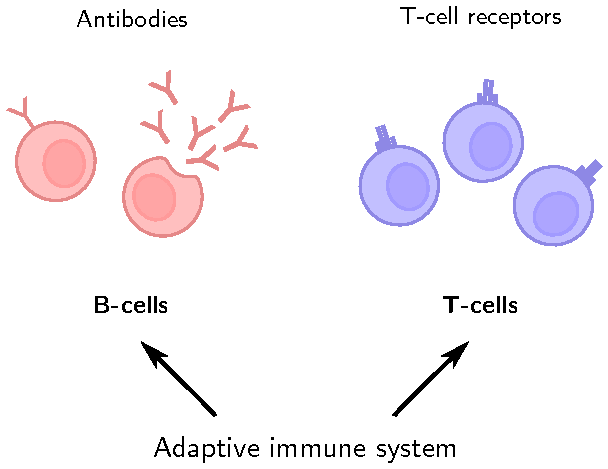
\includegraphics[height=1.1\slideheight]{figs/pdf/adaptive-immunity-simple}
\end{figure}
\end{frame}

\note[itemize]{
\item The adaptive immune system is one of the most complex and sophisticated adaptations in vertebrate biology.
\item By utilising a variety of specialised genome-editing techniques, the population of B-cells and T-cells in the body can collectively express a vast variety of antigen-receptor sequences, allowing them to respond to an almost unlimited range of novel immune challenges.
\item In addition, mechanisms of antigen-dependent clonal expansion and long-lasting immune memory allow the adaptive immune system to rapidly and effectively respond to recurring pathogenic threats, progressively refining its ability to predict and defend against an organism's immune environment.
\item This combination of massive na\"ive sequence diversity on the one hand and adaptive and long-lived immune memory on the other have greatly improved the ability of vertebrates to effectively defend against a complex and rapidly evolving pathogenic ecosystem.
} % TODO: Dario: remove "threats" language?


\begin{frame}
% Slide 3: Adaptive immune ageing
% ~ 1 minute if you talk slowly
\frametitle{Ageing has major effects on human adaptive immunity}\pause
\begin{columns}
\column{0.5\textwidth}
\begin{wideitemize}{0.5}
\item Reduced na\"ive B-cell output
\item Fewer unique antibody sequences
\item Decreased responsiveness to vaccination
\item Impaired antibody quality
\item \dots
\end{wideitemize}\pause
\column{0.5\textwidth}
\begin{figure}
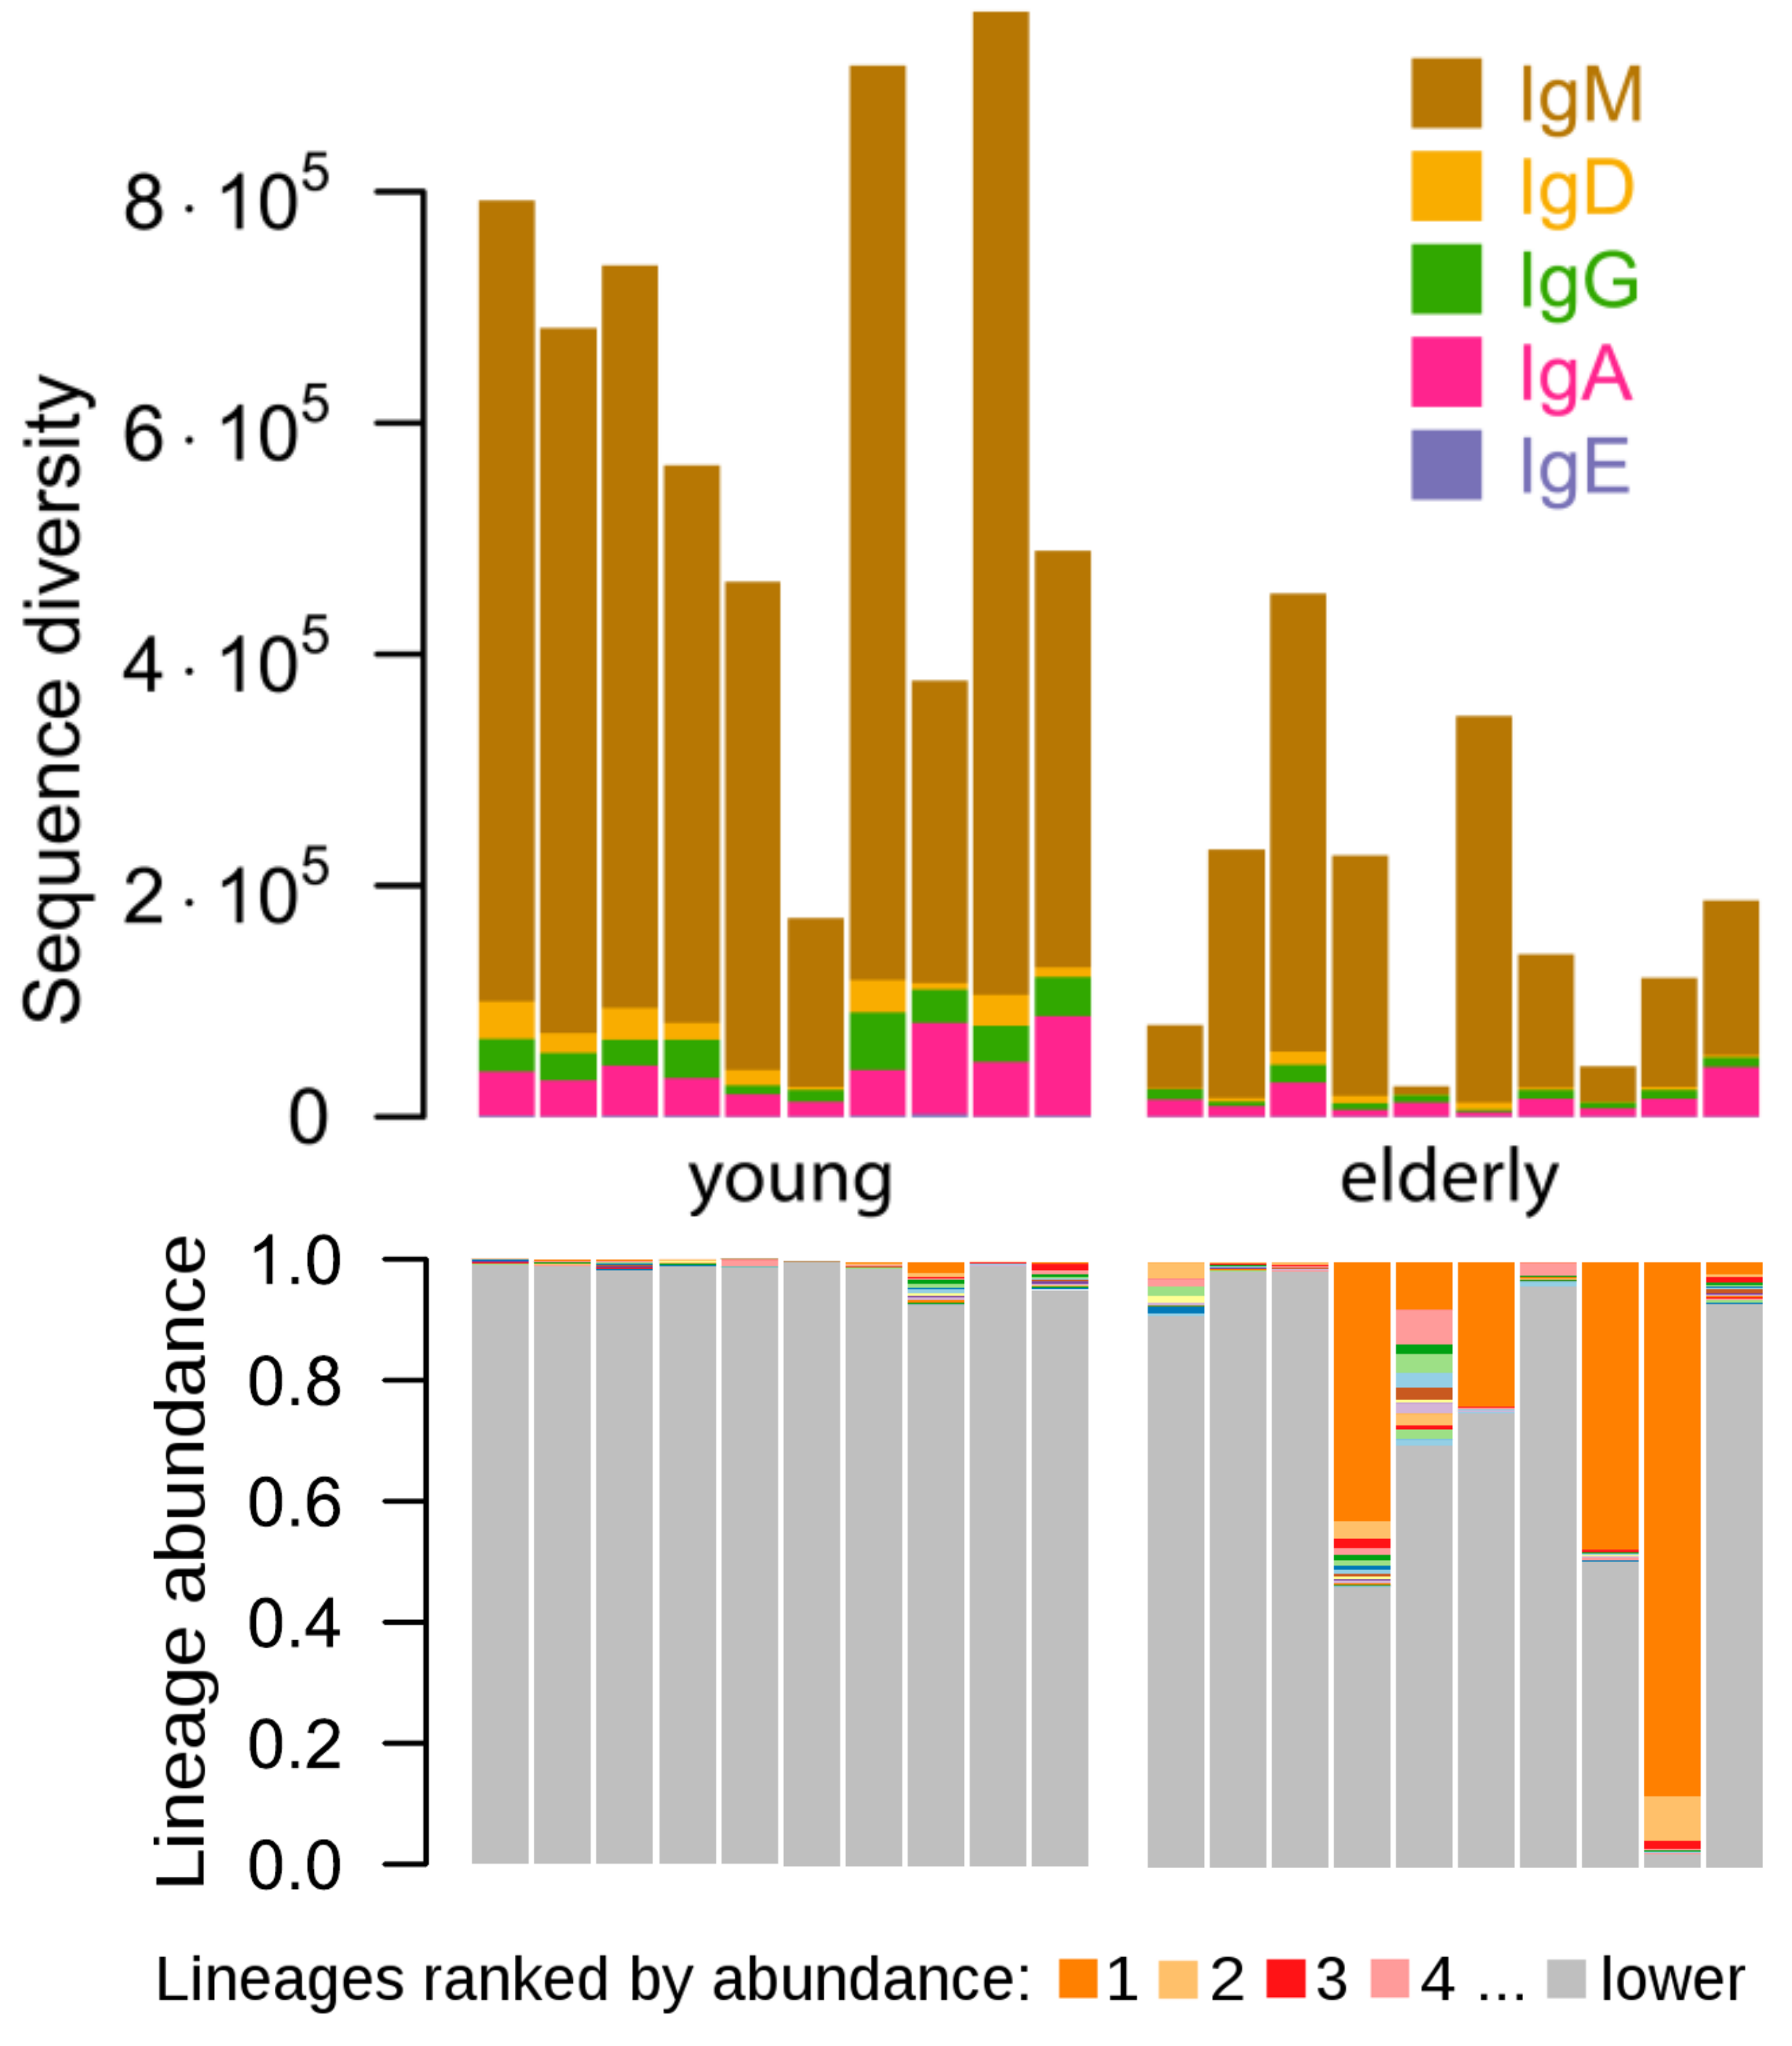
\includegraphics[width=0.90\textwidth]{figs/png/2017_deBourcy_adapted_2groups}
\end{figure}
\begin{flushright}\textit{\scriptsize Adapted from de Bourcey et al., PNAS 2017}\end{flushright}
\end{columns}
\end{frame}

\note[itemize]{
\item Despite all this sophistication, however, the adaptive immune system exhibits dramatic declines in functionality with age.
\item In the case of B-cells, for example, older humans exhibit a wide variety of age-related phenotypes, including reduced production of new na\"ive cells, reduced peripheral sequence diversity, slower and less effective antibody responses to vaccination, and impaired antibody quality.
\item In this study, for example, blood from older humans was found to contain fewer distinct antibody sequences, and more older individuals were found to have B-cell populations disproportionately dominated by the descendents of just a few na\"ive B-cell ancestors.
\item The same study found that the composition of B-cell populations in older individuals was much less flexible, showing significantly less change in response to influenza vaccination.
\item All of this has important implications for immune protection and infection-related morbidity in the elderly
}


\begin{frame}
\frametitle{There's a lot we don't know about adaptive immune ageing}
% Slide 4: What we don't know
% ~ 1.5 minutes
\begin{columns}
\column{0.75\textwidth}\pause
\begin{wideitemize}{0.5}
\item Very little known outside humans and mice\pause
\item Almost all data comes from peripheral blood\pause
\item No spatial resolution (different organs)\pause
\item Limited temporal resolution (typically just two time points)\pause
\item Nothing known about effect of anti-ageing interventions
\end{wideitemize}
\end{columns}
\end{frame} % TODO: Make graphical?
% TODO: Merge resolution points
% TODO: Remove interventions point if not discussing it

\note[itemize]{
\item However, despite this and other studies over several decades there is still a great deal we don't know about the ageing of the adaptive immune system, especially on a quantitative, system-wide level.
\item Most fundamentally, virtually all studies of adaptive immunosenescence have been performed on humans or mice, meaning we know very little about how well these age-related changes are conserved across species or what their evolutionary origins might be.
\item Even within humans, virtually all studies of adaptive immune repertoires -- that is, the collection of antibody or T-cell receptor sequences in an organism -- are performed on peripheral blood samples, which, despite their obvious advantages in terms of non-invasiveness and the ability to conduct longitudinal sampling, are of only limited usefulness as a proxy for the whole-body population of adaptive immune cells.
\item This means that our knowledge of how the adaptive immune system changes with age in particular immune environments (such as at mucosal surfaces) is very limited.
\item In addition to this lack of spatial resolution, the temporal resolution of our knowledge is also restricted -- that is, while we have at least some studies comparing "young" to "old" repertoires, we know much less about the actual kinetics of how these age-related differences accumulate over time.
\item Finally, and unsurprisingly given that most of this work has been done in humans, we know nothing about what experimental interventions might delay or reverse immune repertoire ageing or how such interventions might affect overall healthspan or lifespan.
}



% Slide 5: Models (blackslide + killifish)
% ~ 1.5 minutes
\Blackslide
\note[itemize]{
\item So there are quite a lot of gaps in our knowledge of how adaptive immune repertoires change with age.
\item To fill these gaps we need models -- organisms we can breed at scale, whose biology we can intervene in experimentally, and from which we can obtain and investigate a wide variety of immune organs other than peripheral blood
\item However, for investigating the ageing of a vertebrate-specific adaptation like the adaptive immune system, we've historically been quite restricted in our choice of models: most common vertebrate model systems are quite long-lived (even mice regularly live multiple years) which means investigating or intervening in changes affecting old age in these species is very slow and very expensive.
\item In contrast, most cheap, short-lived model systems that have historically been used for ageing research (such as worms and flies) are not vertebrates and don't have an adaptive immune system.
\item What would be very useful in the immune-ageing field, therefore, is an organism that is both short lived and a vertebrate, with a functioning adaptive immune system.
} % TODO: Remove third figure, revert to killifish growth and wider lifespan

\begin{frame}
\frametitle{The turquoise killifish as a model for antibody ageing}
\begin{figure}
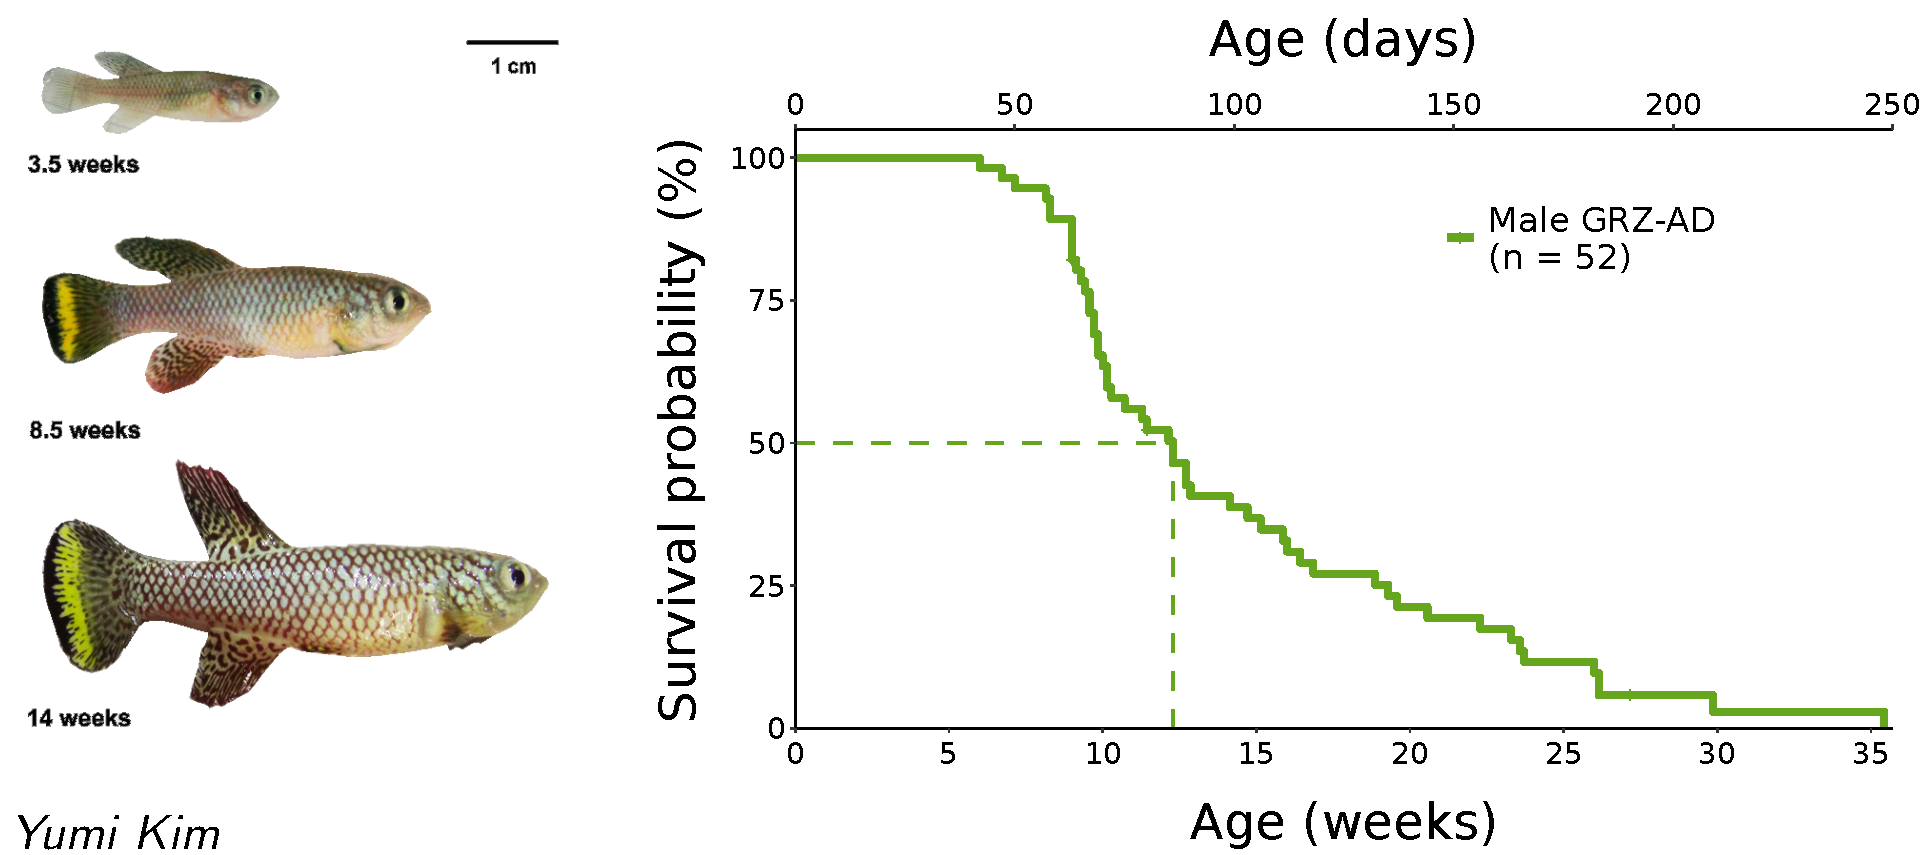
\includegraphics[width=\textwidth]{figs/pdf/intro-turquoise-killifish}
\begin{flushright}\textit{\scriptsize Valenzano et al., Cell 2015}\end{flushright}\vspace{-2ex}
\end{figure}
\begin{wideitemize}{0.5}
\item Shortest-lived vertebrate bred in captivity (median lifespan 12-16 wk)
\item \textbf{Short-lived:} tractable for \alert{large, repeatable ageing experiments}
\item\textbf{Vertebrate:} possesses a \alert{mammal-like adaptive immune system}
\end{wideitemize}
\end{frame}

\note[itemize]{
\item In the Valenzano lab, we've been helping to develop just such a model, namely the turquoise killifish.
\item This is the shortest-lived vertebrate that can be bred in captivity, it's tractable for large, repeatable ageing experiments, and as a teleost fish it possesses a complex, roughly mammal-like adaptive immune system.
\item The combination of all of these traits makes the turquoise killifish a highly promising system for immunosenescence research given some work to establish it as an immunological model.
}

% TODO: Daniel - what is the QUESTION?

\begin{frame}
% Slide 6: The project
% ~ 1 minute
% TODO: Change title to a question
% TODO: Show the locus here? Discuss that you don't have time to go into detail but you characterised it in $n$ species
\frametitle{Understanding adaptive immune ageing in turquoise killifish}
\begin{figure}
\includegraphics<2>[height=1.1\slideheight]{figs/pdf/antibody-structure}
%\includegraphics<3>[width=\textwidth]{figs/pdf/locus-maps} % Show briefly and move on
\end{figure}
\end{frame}

\note[itemize]{
\item During my PhD, therefore, I set out to understand what adaptive immune repertoires looked like in the turquoise killifish and how they changed with age in different contexts
\item To do this, I focused on the immunoglobulin heavy chain, which determines both the majority of the antigen-specificity of an antibody and how it interacts functionally with the rest of the immune system
\item I assembled and characterised the sequence of the heavy-chain gene locus in the turquoise killifish for the first time (that's covered in chapter 3 of my thesis and I'm happy to discuss it more later) and I designed the first working protocol for targeted RNA sequencing of heavy-chain transcripts in this species, adapted to the specialised mechanisms by which mature heavy-chain sequences are produced.
}


% ~ 6 minutes up to here
\begin{frame}
% Slide 7: VDJ recombination and junctional diversity
% ~ 1 minute; could add 1 more sentence here
\frametitle{VDJ recombination and primary antibody diversity}
\begin{figure}
\includegraphics<2>[height=\slideheight]{figs/pdf/vdj-recombination-native}
\includegraphics<3>[height=\slideheight]{figs/pdf/vdj-recombination-select}
\includegraphics<4>[height=\slideheight]{figs/pdf/vdj-recombination-recomb}
\includegraphics<5>[height=\slideheight]{figs/pdf/vdj-recombination-junctions}
\includegraphics<6>[height=\slideheight]{figs/pdf/vdj-recombination}
\end{figure}
\end{frame}

\note[itemize]{
\item In its native state, an immunoglobulin heavy chain locus looks something like this, with blocks of so-called V, D and J gene segments arranged in series on the chromosome.
\item During B-cell development, a single V, D and J segement are selected and the intervening genomic regions are excised to produce a single contiguous VDJ sequence coding for the variable, antigen-binding part of the \textit{IGH} protein.
\item In addition, random insertions and deletions at the VD and DJ junctional boundaries greatly increase the range of possible sequences of the antigen-binding domain.
\item Finally, following transcription, RNA splicing positions this modified VDJ sequence adjacent to the constant region, which codes for the non-variable, structural part of the \textit{IGH} protein chain.
}


\begin{frame}
% Slide 8: TK IgSeq protocol 
% ~ 1 minute
% TODO: Correct arrowhead colour
\frametitle{Immunoglobulin sequencing in the turquoise killifish}
\begin{figure}
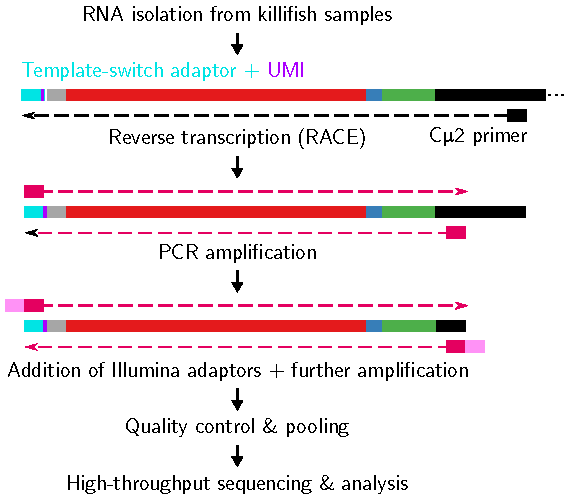
\includegraphics[height=\slideheight]{figs/pdf/igrace-pipeline-wide}
\end{figure}
\end{frame}

\note[itemize]{
\item Therefore, to perform targeted RNA sequencing on the \textit{IGH} variable regions in a killifish sample, the protocol I developed begins with reverse transcription using a gene-specific primer on this constant region, in order to include all the different antigen-binding sequences present in that sample
\item This is followed by several rounds of PCR to amplify the resulting cDNA and attach sequencing adaptors, followed by quality control, pooling and high-throughput sequencing using the Illumina MiSeq system.
\item This is in turn followed by a bioinformatic pre-processing and correction pipeline to convert the initial dataset of error-prone raw reads into a dataset of error-corrected unique sequences, each of which roughly represents the output of a single B-cell present in the original sample.
\item It is this dataset of unique sequences that is used for downstream analysis of the antibody repertoire, including the main question I was looking at in this thesis which was the effect of ageing on repertoire diversity.
}

\begin{frame}
% Slide 9: Ageing cohort sample design
% ~ 1 minute
\frametitle{Sample design -- killifish ageing study}
\begin{figure}
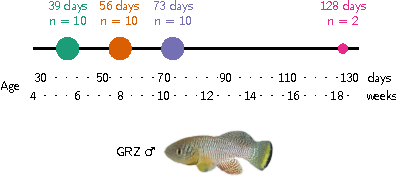
\includegraphics[width=\textwidth]{figs/pdf/design-ageing}
\end{figure}
\end{frame}
% TODO: State ages (new adult, middle aged, etc)

\note[itemize]{
\item In order to investigate this and other effects of ageing on the killifish antibody repertoire, I collected cohorts of adult male turquoise killifish at 39, 56 and 73 days post-hatching, corresponding to 5.5, 8 and 10.5 weeks of age. Some time later I also included two surviving individuals at 128 days post-hatching or 18 weeks of age.
\item All of these fish were sacrificed by anaesthesia, flash-frozen in liquid nitrogen and homogenised prior to total RNA isolation, with the goal of obtaining a representative sample of the whole-body antibody repertoire rather than that of any particular organ.
\item The resulting RNA samples were used as input to the library preparation, sequencing and pre-processing protocol I described in the last slide, to obtain collections of unique \textit{IGH} variable region sequences for each individual in each age group
\item This gave me a dataset I could use to compare the diversity and structure of the antibody repertoires between killifish of different ages
}

\begin{frame}
% Slide 10: Explaining clonal diversity
% ~ 1 minute
\frametitle{Clonal antibody diversity}
\begin{figure}
\includegraphics<2>[width=\textwidth]{figs/pdf/clonal-expansion-1}
\includegraphics<3>[width=\textwidth]{figs/pdf/clonal-expansion-2}
\includegraphics<4>[width=0.95\textwidth]{figs/pdf/clonal-diversity-groups}
\end{figure}
\end{frame}
% TODO: Dario - label naive cells, clones etc. labels

\note[itemize]{
\item The first thing I looked at was the effect of ageing on the clonal diversity of the repertoire
\item I mentioned at the start of this talk that B-cells undergo clonal expansion following antigen exposure, and during this clonal expansion the antigen-binding domain sequences of proliferating B-cells undergo very high rates of somatic mutation, resulting in a family of B-cells descended from a single ancestral cell expressing similar but non-identical antigen-binding sequences.
\item This is referred to as a B-cell clone.
\item The size of these clones can vary dramatically: many na\"ive B-cells will never encounter antigen and so have very few descendents, while a few B-cell lineages will be repeatedly and strongly stimulated by antigen resulting in very large clones containing many thousands or even more individual cells.
\item The clonal diversity of a repertoire measures both the number of clones and the degree to which these clones differ in size, with a repertoire containing more clones or more evenly-distributed clone sizes considered more diverse.
}

\section{Results}

\begin{frame}
% Slide 11: Clonal alpha diversity results
% ~ 2.5 minutes if take it slow
\frametitle{Clonal alpha diversity in the killifish antibody repertoire \only<2->{declines with age \only<3->{at high diversity orders}}}
\begin{figure}
\includegraphics<2>[height=\slideheight]{figs/pdf/ageing-clone-diversity-alpha}
\includegraphics<3>[width=0.9\textwidth]{figs/pdf/ageing-clone-diversity-solo-fit-gamma}
\end{figure}
\end{frame} % TODO: Add text for Hill numbers, reminder that 0 -> 1 = less -> more downweighting
% TODO: Add arrow showing direction of diversity change with age
% TODO: Emphasise speed of diversity loss
% TODO: Restore colour legend

\note[itemize]{
\item So, what do clonal diversity measures tell us about antibody repertoire ageing in the turquoise killifish?
\item This is a plot of the clonal diversity spectrum of each age group in the dataset from 5.5 to 18 weeks. Each curve gives the alpha diversity (that is, roughly, the average within-repertoire diversity across all individuals) for a single age group across many different diversity measures differing in their diversity order $q$. 
\item This order of diversity refers to how strongly rare clones are discounted relative to common ones when calculating the diversity -- at order zero, all clones are counted equally, while at high order only the most common clones contribute to the diversity measurement.
\item This means that each position along the $x$-axis captures a different aspect of the diversity structure of each population.
\item In the case of the killifish dataset we can see a pretty clear decline in clonal diversity with age across most of the range of diversity orders we consider: from about order 1 upwards the diversity of the 5.5-week-old group is higher than that of the 8-week-old group, which in turn is much higher than either of the older groups, which overlap in diversity with each other
\item This suggests that, at least for higher-order alpha diversity, the clonal repertoire of turquoise killifish becomes less diverse with age
\item <change frame> To test the significance of this observation, I selected six individual diversity orders (0, 1, 1.5, 2, 3, and 4), fit a Gamma-distributed generalised linear model to the individual diversity measurements of the individuals in each age group, and tested the significance of the ageing term
\item The results indicate that there is a significant decline in clonal antibody diversity with age at diversity order 1.5 or higher, but not at low orders below 1.5. 
\item Since higher order measurements are dominated by large clones but low-order measurements are dominated by small clones (which are much more numerous) this suggests that in the turquoise killifish, the diversity of large, expanded clones in the repertoire declines with age while that of small, unexpanded clones does not change significantly.
}

% Slide 12: Explain VJ diversity and results
\begin{frame}
% ~ 1 minute if take it slow
% TODO: Mention why VJ and not VDJ here
\frametitle{\textbf{VJ} alpha diversity in the killifish antibody repertoire \only<10->{\textbf{does not decline} with age}}
\begin{figure}
\includegraphics<1>[height=0.95\slideheight]{figs/pdf/vj-diversity-cell0}
\includegraphics<2>[height=0.95\slideheight]{figs/pdf/vj-diversity-cell1}
\includegraphics<3>[height=0.95\slideheight]{figs/pdf/vj-diversity-cell2}
\includegraphics<4>[height=0.95\slideheight]{figs/pdf/vj-diversity-cell3}
\includegraphics<5>[height=0.95\slideheight]{figs/pdf/vj-diversity-cell4}
\includegraphics<6>[height=0.95\slideheight]{figs/pdf/vj-diversity-cell5}
\includegraphics<7>[height=0.95\slideheight]{figs/pdf/vj-diversity-clones}
\includegraphics<8>[height=0.95\slideheight]{figs/pdf/vj-diversity-groups}
\includegraphics<10>[height=0.95\slideheight]{figs/pdf/ageing-vj-diversity-alpha}
\includegraphics<11>[height=0.95\slideheight]{figs/pdf/ageing-vj-diversity-alpha-sig}
\end{figure}
\end{frame}

\note[itemize]{
\item Partitioning the antibody repertoire into clones is one way of looking at repertoire diversity. Another is to look at the choices made by B-cells during VDJ recombination by quantifying the diversity of different V/J combinations present in the repertoire.
\item In this method, sequences are partitioned based on their V and J identities rather than their clonal identity, meaning that cells from different clones whose ancestors chose the same V and J segments during VDJ recombination will be grouped together.
\item If we investigate the diversity of V/J selection groups in this way, we see a very different pattern from the one we saw for clonal diversity: there is no apparent difference in the diversity spectra between different age groups, and if we test for a significant age effect using GLMs as before we find no significant difference at any diversity order.
}

\Blackslide
% Slide 13: Difference between clonal and VJ diversity (black)
% ~ 1 minute

\begin{frame}
\frametitle{So does the killifish antibody repertoire decline in diversity with age?}
\begin{wideitemize}{1.5}\pause\Large
\item \textbf{Yes} (clonal diversity)\pause
\item \textbf{No} (V/J diversity)\pause\vspace{1em}
\item Why the difference?
\end{wideitemize}
\end{frame}
% TODO: Blackslide for puzzle, graphical slide for model

\note[itemize]{
\item So it seems like the answer to the question ``does the killifish antibody repertoire decline in diversity with age'' doesn't really have a straight answer -- it does if you mean clonal diversity, but not if you mean V/J segment-usage diversity.
\item This seems surprising and a bit odd -- why would you see a significant loss of diversity with age if you partition the sequences in the repertoire one way, but not in a different but related way?
\item In the end I decided that the difference probably had something to do with the fact that clonal diversity was declining significantly at high but not low diversity orders. If the repertoire is dominated at all ages by large numbers of small clones, whose statistical properties don't change much with age (resulting in no change in low-order clonal diversity), then the lack of change in V/J usage with age in these small clones could outweigh whatever changes are occurring in the minority of expanded clones, resulting in no significant change to the overall V/J diversity of the repertoire.
\item If this is the explanation, then we would expect that sequences contained within large clones would show a significant decline in VJ diversity with age, even though the entire population of sequences does not
}

\begin{frame}
% Slide 14: VJ diversity of large clones
% ~ 1 minute if take it slow; could add another figure/sentence or two or split into two slides
\frametitle{\textbf{VJ} alpha diversity of \textbf{large clones} \only<2->{\textbf{does decline} with age}}
\begin{figure}
\includegraphics<2>[height=0.95\slideheight]{figs/pdf/ageing-vj-diversity-vlarge-alpha}
\includegraphics<3>[height=0.95\slideheight]{figs/pdf/ageing-vj-diversity-vlarge-alpha-sig}
\end{figure}
\end{frame}

\note[itemize]{
\item To test this prediction, I filtered the killifish dataset to only those sequences contained in clones with at least five unique sequences and repeated the V/J diversity calculation on this restricted set
\item In sharp contrast to the results for the entire dataset, sequences from large clones showed a dramatic decline in V/J diversity with age, which was significant across the entire range of diversity orders
\item This is consistent with the results from the clonal diversity analysis
\item This goes quite some way in supporting a model in which the killifish antibody repertoire can be partitioned into a very large number of small, unexpanded clones which do not change significantly in their statistical composition with age, and a much smaller group of large, expanded clones which exhibit a strong, age-related decline in repertoire diversity
}

% TODO: Make clear that small clones = mainly naive, unexperienced clones, while large clones = stimulated, expanded clones
% TODO: Write down somewhere that large = 5 or more sequences

% ~ 15.5 minutes up to here

\Blackslide

% Slide 15: Beta diversity
\begin{frame}
\frametitle{Killifish VJ repertoires become \textbf{more dissimilar} with age}
\begin{figure}
\includegraphics<1>[width=\textwidth]{figs/pdf/ageing-vj-diversity-beta}
\includegraphics<2>[width=\textwidth]{figs/pdf/ageing-rdi}
\end{figure} % TODO: Add note that RDI = repertoire dissimilarity index
\end{frame}
% TODO: Restore colour legend
% TODO: Take out KWT p-value
% TODO: Add "days" to PCoA plot

\note[itemize]{
\item So far we've only discussed alpha diversity, which measures the average within-individual diversity of a group of repertoires and compares this between groups
\item Another way to conceptualise the diversity of a group of repertoires is the beta diversity, which measures the extent to which repertoires in a group differ from each other
\item Beta diversity can't be measured for clonal diversity as by definition each clone is unique to an individual and so each pair of repertoires is maximally different in composition. However, the range of possible V/J choices is shared between individuals and so the degree to which repertoires are similar or different in their V/J composition can be measured and compared between age groups.
\item One way to present this is using a beta diversity spectrum, which is similar in conception to an alpha-spectrum: higher $y$-values indicate more divergence between individuals, while higher $x$-values indicate a greater relative downweighting of rare V/J-combinations relative to common ones. Depicting the results in this way, we see that beta diversity increases dramatically with age, especially at high diversity orders and regardless of whether all clones or only large clones are included.
\item This indicates that as turquoise killifish individuals age they become more and more distinct in the V/J composition of their antibody repertoires
\item <change figures> Another way to analyse the same phenomenon is the repertoire dissimilarity index, which is derived from the Euclidean distance between the V/J usage vectors of different repertoires and gives a pairwise distance measure between any two individuals. If we look at the distribution of RDI distances in each group we again see a progressive increase in the median pairwise distance between individuals in older groups. If we visualise this in two dimensions using a principal co-ordinate analysis, this increase can be seen as a progressive drifting apart as individuals grow older, suggesting again that each individual's antibody repertoire becomes more distinct and individualised as it ages.
}

% Slide 16: Whole body summary
% TODO: Emphasise AGEING up front
% TODO: Make a graphical summary
% TODO: Try to explicitly reconcile summary with gap/question
\begin{frame}
\frametitle{Summary I}
\begin{wideitemize}{0.5}\pause
\item Antibody repertoires sampled from whole-body killifish samples show a progressive decline in clonal alpha diversity at high (but not low) diversity orders\pause
\item V/J alpha diversity shows no change with age if all clones are included but a large decline in large clones\pause
\item Between-individual variation (beta diversity) in killifish repertoires increases with age
\end{wideitemize}
\end{frame}

\note[itemize]{
\item In summary, therefore, antibody repertoires sampled from whole-body turquoise-killifish samples show a progressive decline in clonal alpha diversity at high but not at low diversity orders, indicating a loss of antibody diversity concentrated in the minority of large expanded clones.
\item The V/J alpha diversity of these repertoires shows no change with age if all clones are included, but a large age-related decline if only sequences from large clones are considered, supporting the hypothesis that age-related effects on diversity differ between small and large clones.
\item Finally, both beta diversity spectra and RDI measures show that the between-individual variation in V/J usage in the turquoise killifish increases with age, indicating that the killifish antibody repertoire becomes more distinct and individualised as individuals get older.
\item Collectively, these findings show that the composition of the antibody repertoire in the turquoise killifish undergoes complex and important changes over the course of adulthood, with potentially important implications for immune functionality.
}

\Blackslide

% Slide 17: Intro to gut stuff
\begin{frame}
\frametitle{Killifish gut microbiota also show decreasing alpha- and increasing beta diversity with age}
\begin{figure}
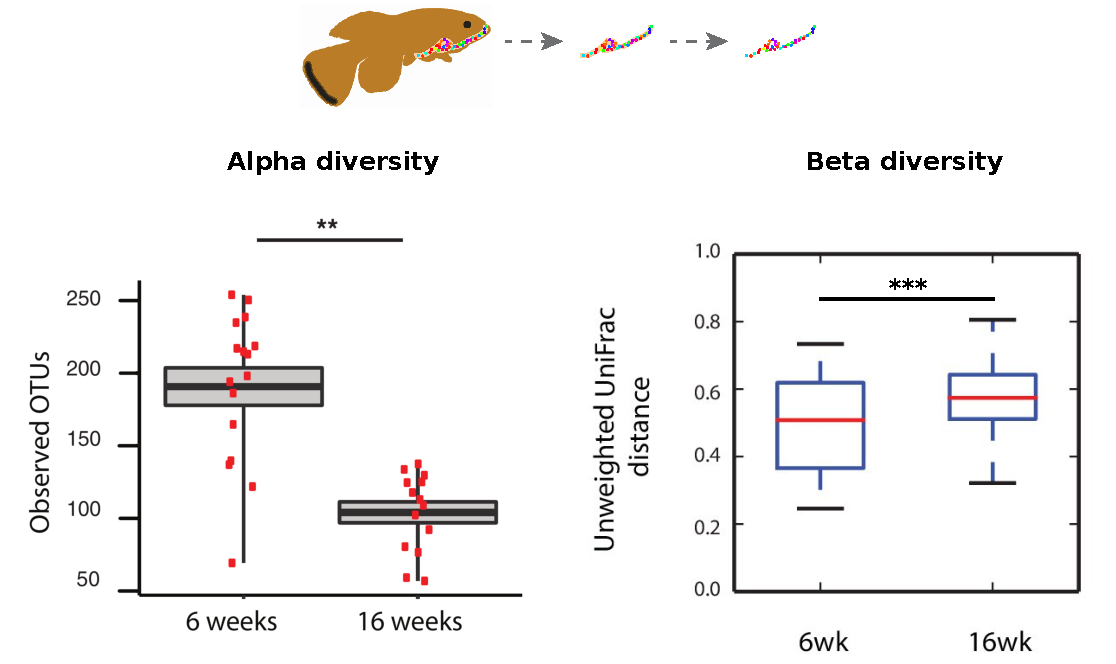
\includegraphics[width=0.85\textwidth]{figs/pdf/microbiota-diversity}
\attrib{Smith et al., eLife 2017}
\end{figure}
\end{frame}

\note[itemize]{
\item This isn't the first time in the turquoise killifish that we've seen a decline in within-individual diversity and an increase in between-individual variability with age.
\item Earlier published work from the Valenzano lab has shown that the killifish gut microbiota also follows this pattern, with older fish exhibiting a less diverse microbiota whose composition is more variable between individuals.
\item Given the importance of intestinal B-cell populations in regulating gut microbiotal composition, and the fact that no one has previously investigated the effect of ageing on intestinal antibody repertoires specifically, I decided to investigate how repertoire diversity in the gut (as opposed to the entire body) changes with age.
}

% Slide 18: Gut sample design
\begin{frame}
\frametitle{Sample design -- gut repertoire study}
\begin{figure}
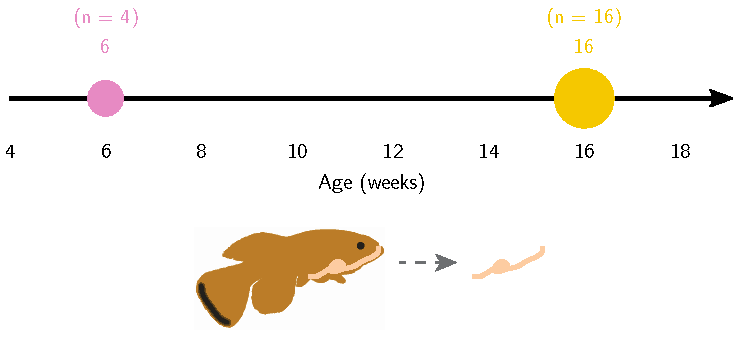
\includegraphics[width=\textwidth]{figs/pdf/design-gut}
\end{figure}
\attrib{Samples collected for Smith et al., eLife 2017}
\end{frame}

\note[itemize]{
\item To do this, we made use of gut total RNA samples collected from adult male turquoise killifish as part of the microbiota study at either 6 or 16 weeks post-hatching.
\item These RNA samples underwent the same library preparation protocol I described earlier, which in this case was performed by Michael Poeschla and Aleksandra Placzek, both of whom are in the audience today. The resulting libraries were sequenced and pre-processed as I described for whole-body samples, resulting in a collection of unique variable-region sequences for each individual.
\item I could then use these sequences to quantify the alpha and beta repertoire diversities as I described before, but this time for intestinal rather than whole-body B-cell populations.
}

% Slide 19: Gut beta diversity
\begin{frame}
\frametitle{Killifish gut repertoires become much more dissimilar with age}
\begin{figure}
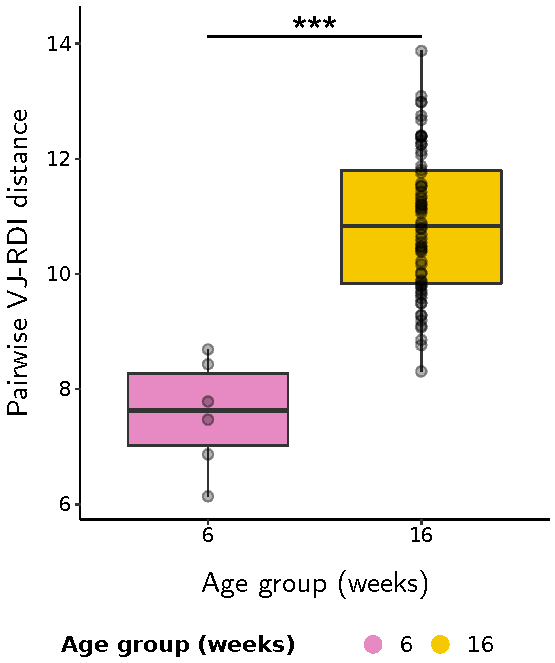
\includegraphics[width=\textwidth]{figs/pdf/igseq-gut-rdi}
\end{figure} % TODO: Add note that RDI = repertoire dissimilarity index
\end{frame} % TODO: *VJ*-RDI distance

\note[itemize]{
\item First of all, the between-individual variability of the gut repertoires again increased with age, in a pattern broadly similar to that seen in whole-body repertoires.
\item Here I show the results from the repertoire dissimilarity index, which again shows a higher median between-individual distance in older individuals corresponding to a spreading-out of points in a principal co-ordinate analysis.
\item In this respect, gut repertoires don't seem to differ overmuch from those of the whole body.
}

% Slide 20: Gut alpha diversity
\begin{frame}
\frametitle{Gut repertoire alpha diversity declines dramatically with age in turquoise killifish}
\begin{figure}
\includegraphics<1,3>[width=\textwidth]{figs/pdf/igseq-gut-combined-diversity-alpha}
\includegraphics<2>[width=\textwidth]{figs/pdf/igseq-ageing-combined-diversity-alpha}
\end{figure}
\end{frame}

\note[itemize]{
\item Conversely, however, the effect of ageing on the alpha diversity of the gut repertoire is much more dramatic than in the whole body
\item Both the clonal and V/J alpha diversity spectra show large differences between the six- and sixteen-week old groups, which are highly significant under the GLM-based test I described before.
\item <change figure> Just as a reminder, this is what the equivalent plots from the whole-body dataset looks like
\item <change figure> It's really quite a dramatic difference in the apparent size and significance of the age effect.
\item And this suggests that gut mucosal antibody repertoires in turquoise killifish are undergoing a much stronger loss of alpha diversity with age than is seen in the whole-body repertoire overall
}

% Slide 21: Explanations for difference
\begin{frame}
\frametitle{Why the difference?}
\Large
\begin{wideenum}{1}\pause
\item Difference in \textbf{environment}?\vspace{0.5em}
\begin{wideitemize}{0.5}\pause
\item Intense antigen exposure from gut microbiota
\item Greater antigen exposure $\to$ more clonal expansion, less diversity\pause
\end{wideitemize}
\item Difference in \textbf{clonal composition}?\vspace{0.5em}
\begin{wideitemize}{0.5}\pause
\item Whole body includes primary lymphoid organs, intestine does not
\item $\to$ More small na\"ive clones in whole-body samples than gut samples
\item Larger clones more age-sensitive $\to$ stronger age effect in gut samples
\end{wideitemize}
\end{wideenum}
\end{frame}

\note[itemize]{
\item What might be causing this difference?
\item One possibility is that it's a result of the unique environment these B-cells find themselves in, with constant intense antigen exposure from the gut microbiota resulting in ever-increasing levels of clonal expansion and hence reduced alpha diversity. This might well be true, but it's not really something I could test with the data I have available at present.
\item Another possibility, which is not mutually exclusive with the first, is that the difference has to do with the composition of different B-cell subpopulations in whole-body and mucosal repertoires. The whole-body samples include B-cells from the primary lymphoid organs where new nai\"ve B-cells are produced, and therefore contain very large numbers of small B-cell clones that have never encountered antigen. In contrast, the gut samples only contain B-cells that have migrated from the primary lymphoid organs or elsewhere to become resident in the intestine. As such, gut repertoires may contain a much smaller proportion of small clones relative to whole-body repertoires. Since as we saw before large clones show a much stronger age-related change in repertoire diversity compared to small clones, this might be enough to explain some or all of the difference between the two sets of results.
}

\Blackslide

% Slide 22: Rarefaction
\begin{frame}
\frametitle{Killifish gut repertoires contain fewer \textbf{small} clones than whole-body repertoires}
\begin{figure}
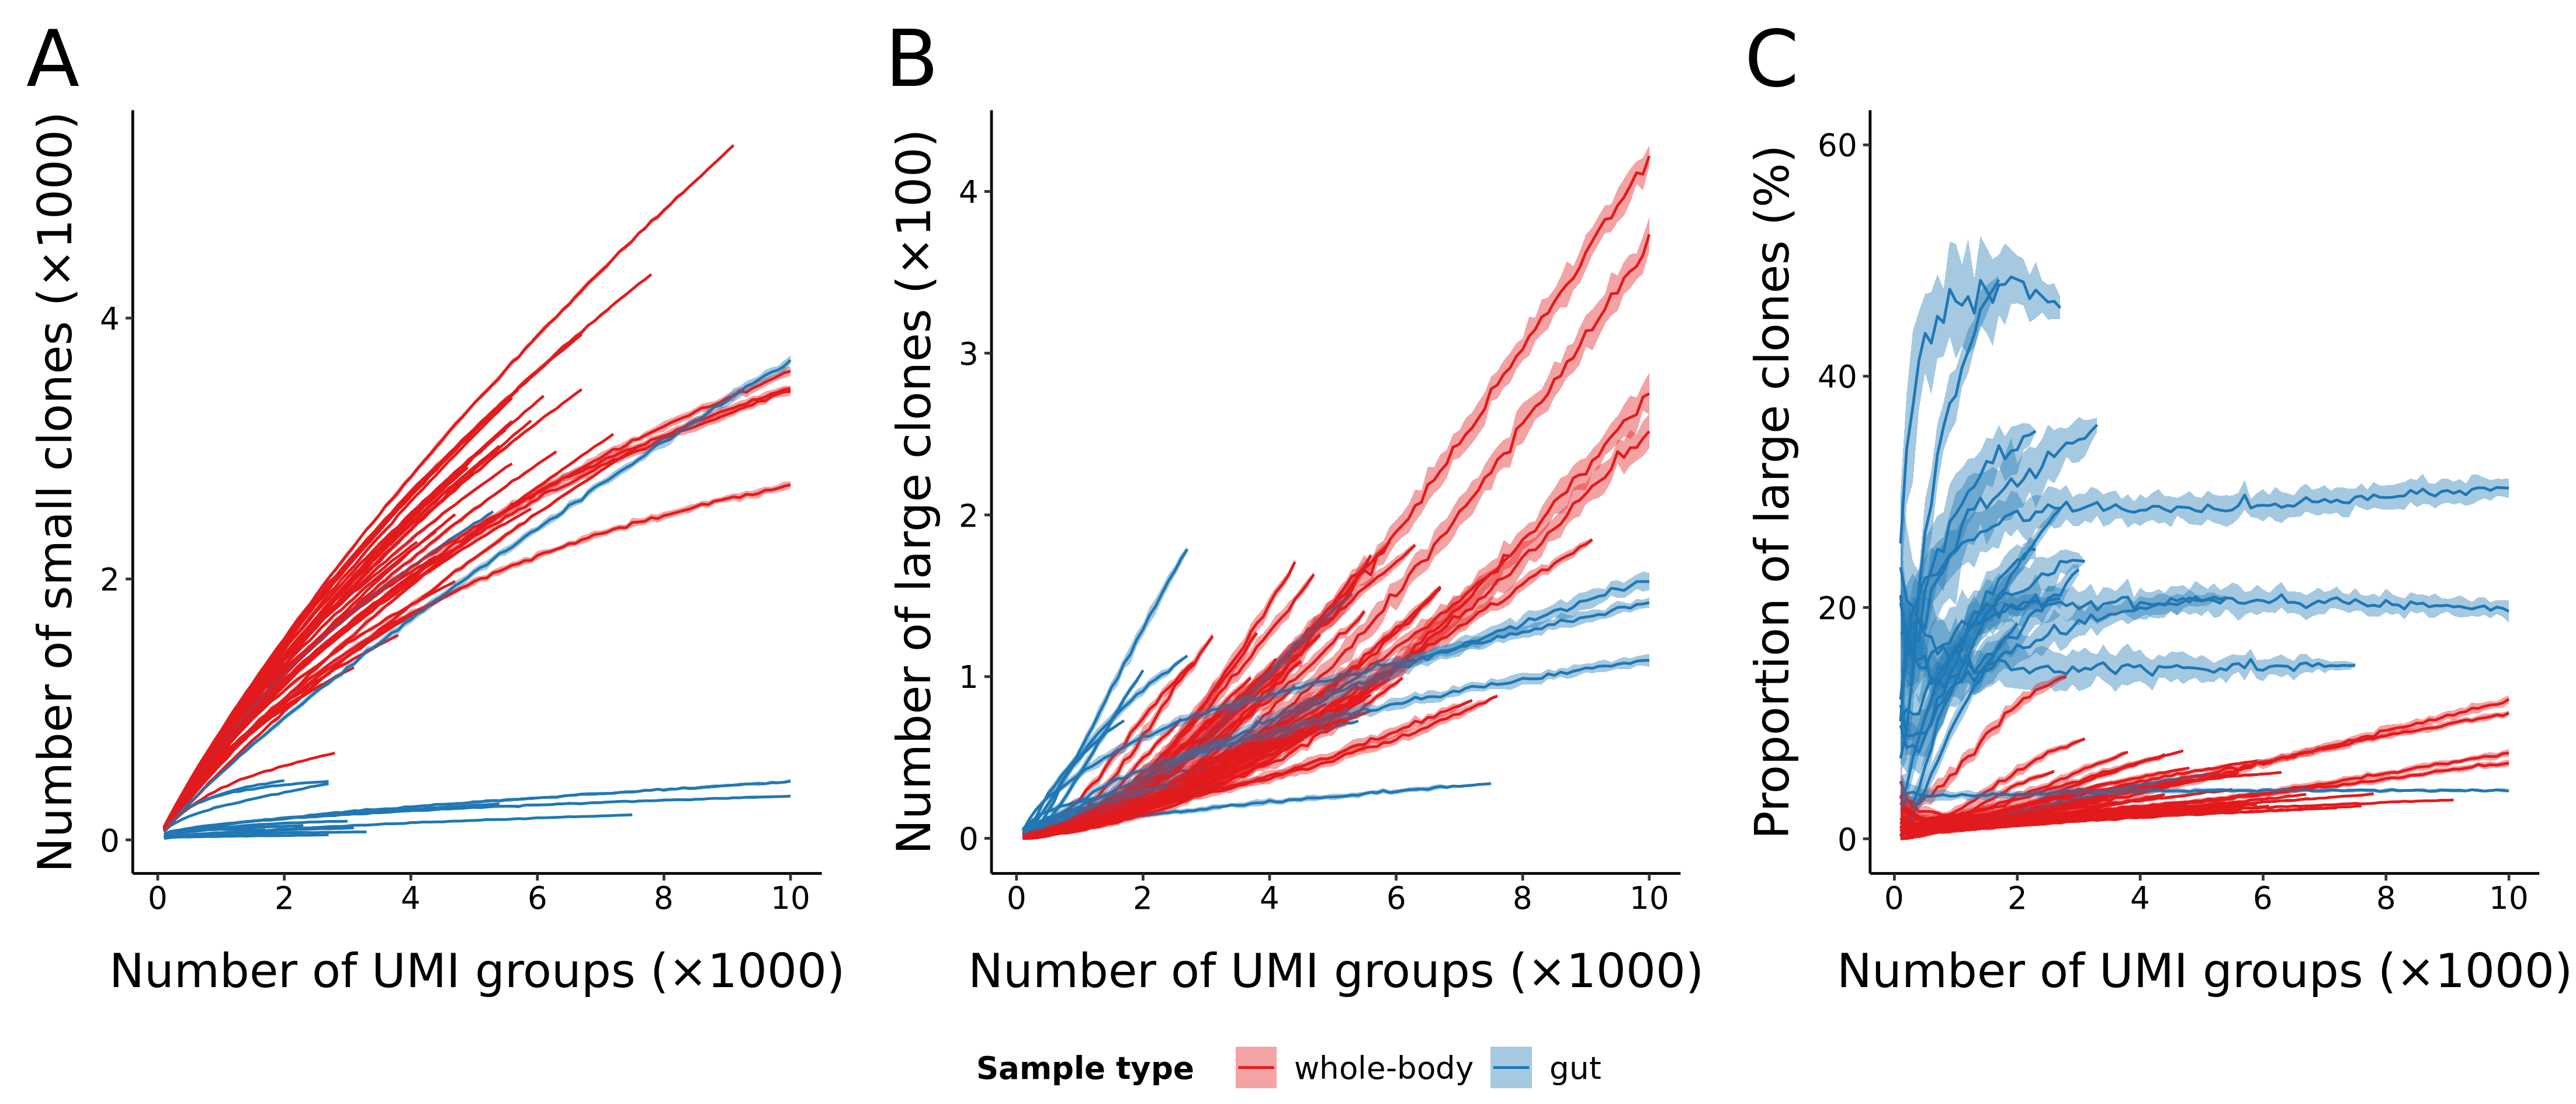
\includegraphics[width = \textwidth]{../_Figures/png/igseq-rarefied-clone-2colour-counts-size.png}
\end{figure}
\end{frame}

\note[itemize]{
\item So, is it in fact the case that killifish gut repertoires contain a smaller proportion of small clones than whole-body repertoires do?
\item To test this, I made use of rarefaction analysis, in which I repeatedly downsampled each repertoire in each dataset down to a certain number of sequences and counted the number of small and large and total clones at each sample size, as well as the relative proportion of large versus small clones.
 \item This allowed the gut and whole-body samples to be compared in a more representative manner
\item The results showed a quite dramatic difference between the two datasets, with most intestinal samples containing many fewer small clones than most whole-body samples but a much more similar number of large clones, resulting in a much higher relative prevalence of large clones in the repertoire.
\item This supports a model in which the much more dramatic declines in repertoire alpha diversity with age in gut samples are at least partly due to the fact that these samples contain a greater proportion of (apparently more age-sensitive) large clones
}

% Dario: include slide with relative decline rate statistics?

% Slide 23: Summary II
\begin{frame}
\frametitle{Summary II}\pause
\begin{wideitemize}{0.5}
\item The turquoise killifish is a highly promising model system for immune ageing research\pause
\item A complete \textit{IGH} locus structure and IgSeq library-prep protocol are now available in killifish for the first time\pause
\item Large (but not small) killifish B-cell clones show a significant decline in antibody alpha diversity with age in whole-body samples\pause
\item Killifish intestinal samples show a much more dramatic decline in alpha diversity with age than in the whole body\pause
\item Both gut and whole-body repertoires show an increase in beta diversity with age
\end{wideitemize}
\end{frame}
% TODO: Dario - key points:
% 1. You observe repertoire ageing in the killifish
% 2. How does repertoire ageing occur?

\note[itemize]{
\item The turquoise killifish is a highly promising model system for investigating adaptive immunosenescence due to its short lifespan and mammal-like adaptive immune system
\item As a result of the work done during my time in the Valenzano lab, a complete \textit{IGH} locus structure and working library preparation protocol for immunoglobulin sequencing are now available for the turquoise killifish, establishing it for the first time as a new ready-to-use model for quantitative immunology
\item Quantification of antibody repertoire diversity in whole-body samples suggests that large B-cell clones undergo a significant decline in repertoire diversity with age, while small antigen-inexperienced clones do not appear to change significantly in this respect. More work is needed to ascertain why this is the case and what consequences it has for killifish adaptive immunity.
\item In the killifish intestine, gut mucosal B-cells undergo a much more dramatic decline in alpha diversity with age than the whole body population, a difference at least partially attributable to the fact that mucosal B-cell populations are relatively more dominated by large, age-sensitive clones. To my knowledge, this is the first time the ageing of mucosal antibody repertoires has been formally investigated in this way.
\item Finally, while the alpha diversity decreases, the beta or between-individual diversity increases significantly with age in both whole-body and gut mucosal repertoires, indicating that, as in humans, older killifish acquire a progressively more individualised and distinct antibody repertoire as they age. 
\item Together, these results demonstrate the value of the turquoise killifish as a model for adaptive immune ageing and lay the groundwork for future investigation of the interaction between microbiota and adaptive-immune ageing and the effect of experimental interventions on the ageing of the antibody repertoire.
}

% Slide 24: Acknowledgements
%\section{Acknowledgements}
%
\begin{frame}
\frametitle{Acknowledgements}
\small
\begin{columns}
\column{0.25\textwidth}
Dario Valenzano\\
\alert{Aleksandra Placzek}\\
\alert{Davina Patel}\\
\alert{Michael Poeschla}\\
Ray Cui\\
Joanna Dodzian\\
\alert{Pascha Hokama}\\
\alert{Lena Schlautmann}\\\vspace{1.7ex}
All other DV lab members\\\vspace{1.7ex}
Daniela Morick\\
Doris Birker\\
Jenny Ostermann\\\vspace{1.7ex}
Aleksandra Walczak\\
B\'{e}r\'{e}nice Benayoun\\
John Beausang
\column{0.75\textwidth}
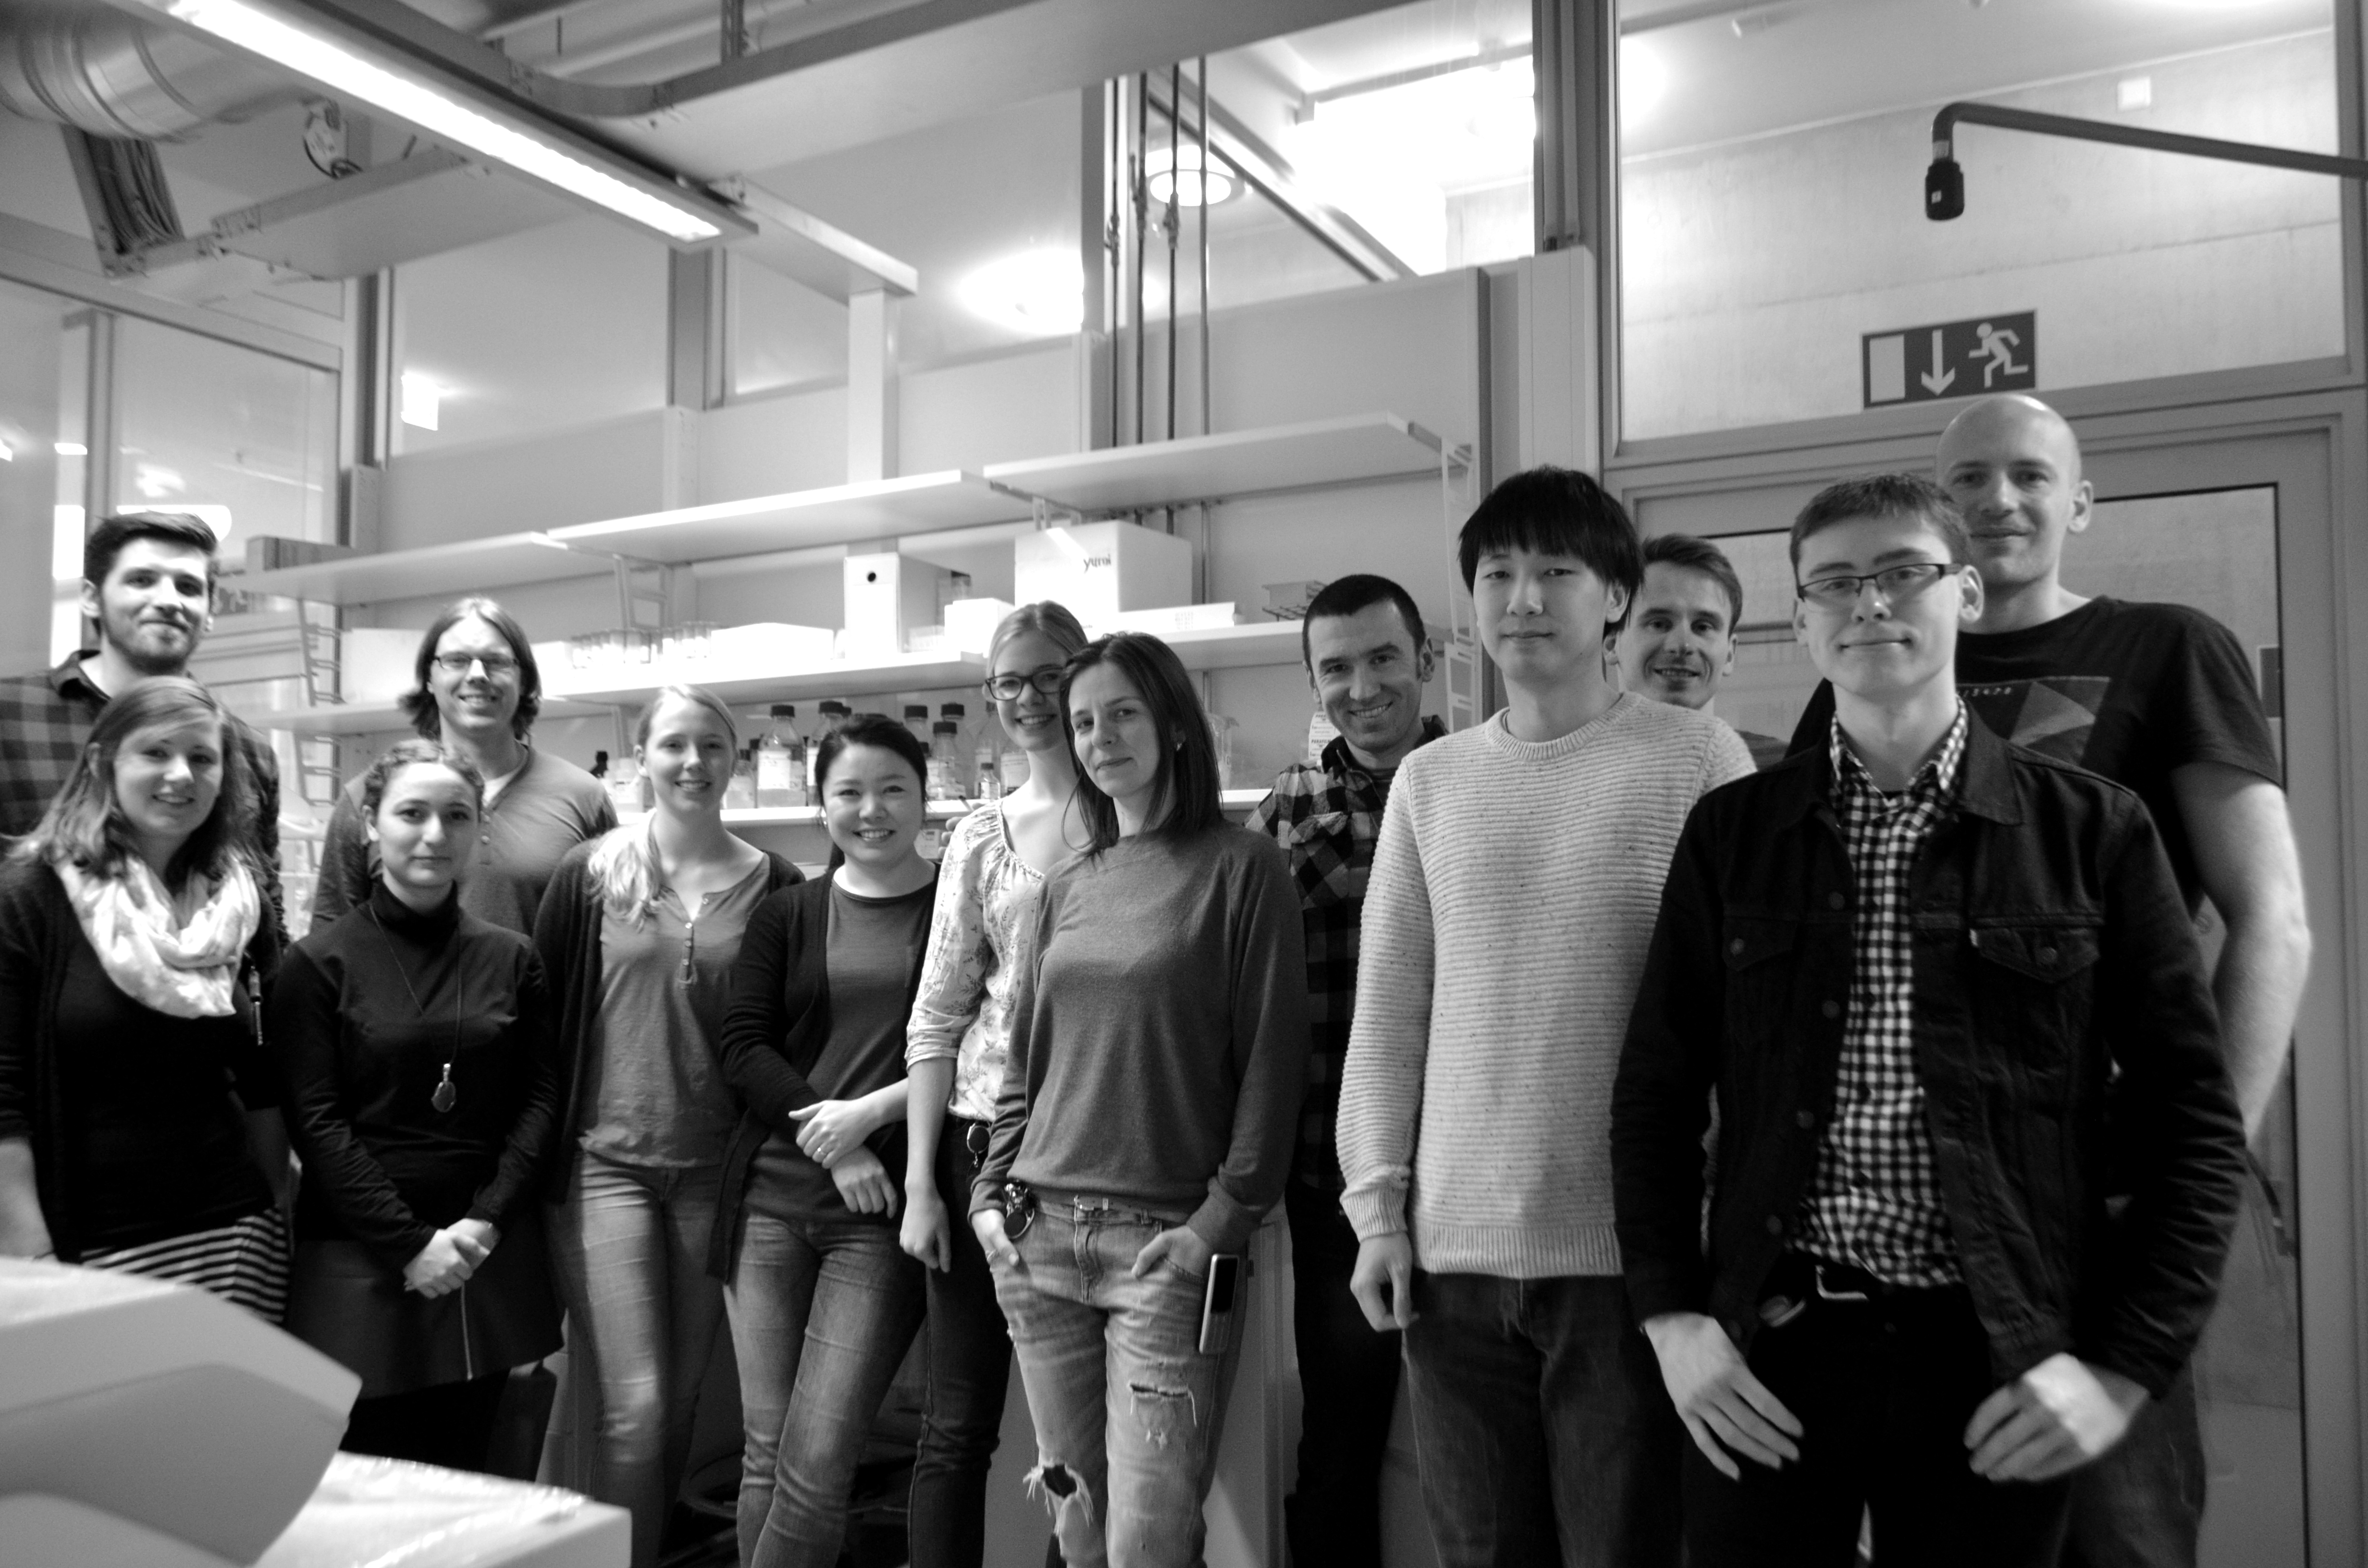
\includegraphics[width=\textwidth]{figs/jpg/group-2016}\vspace{1em}\\
\begin{columns}
\column{0.37\textwidth}
Kathrin Reichwald\\
Jason Vander Heiden\\
Quentin Marcou
\column{0.38\textwidth}
Manolis Pasparakis\\
Andreas Beyer\\
Michael L\"assig\\
\end{columns}
\end{columns}
\end{frame}
%
% % Slide 25: Thank you and questions

\section{}
\begin{frame}\begin{center}
\Huge Thank you!
\end{center}\end{frame}


% -----------------------------------------------------------------------------


\appendix
\blackslide
\section*{Extra slides}

%\begin{frame}
%\frametitle{Primary and secondary antibody diversity}
%\begin{figure}
%\includegraphics<1>[height=\slideheight]{figs/pdf/bcell-repertoire-naive}
%\includegraphics<2>[height=\slideheight]{figs/pdf/bcell-repertoire-primary}
%\includegraphics<3>[height=\slideheight]{figs/pdf/bcell-repertoire-derived}
%\includegraphics<4>[height=\slideheight]{figs/pdf/bcell-repertoire-primary-secondary}
%\end{figure}
%\end{frame}


\begin{frame}
\frametitle{Bioinformatics pipeline}
\begin{figure}
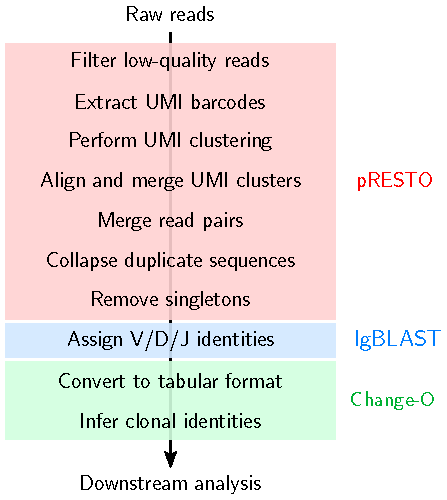
\includegraphics[height=\slideheight]{figs/pdf/immcantation-pipeline}
\end{figure}
\end{frame}

\begin{frame}
\frametitle{The generative entropy of the na\"ive antibody repertoire does not change with age}
\begin{figure}
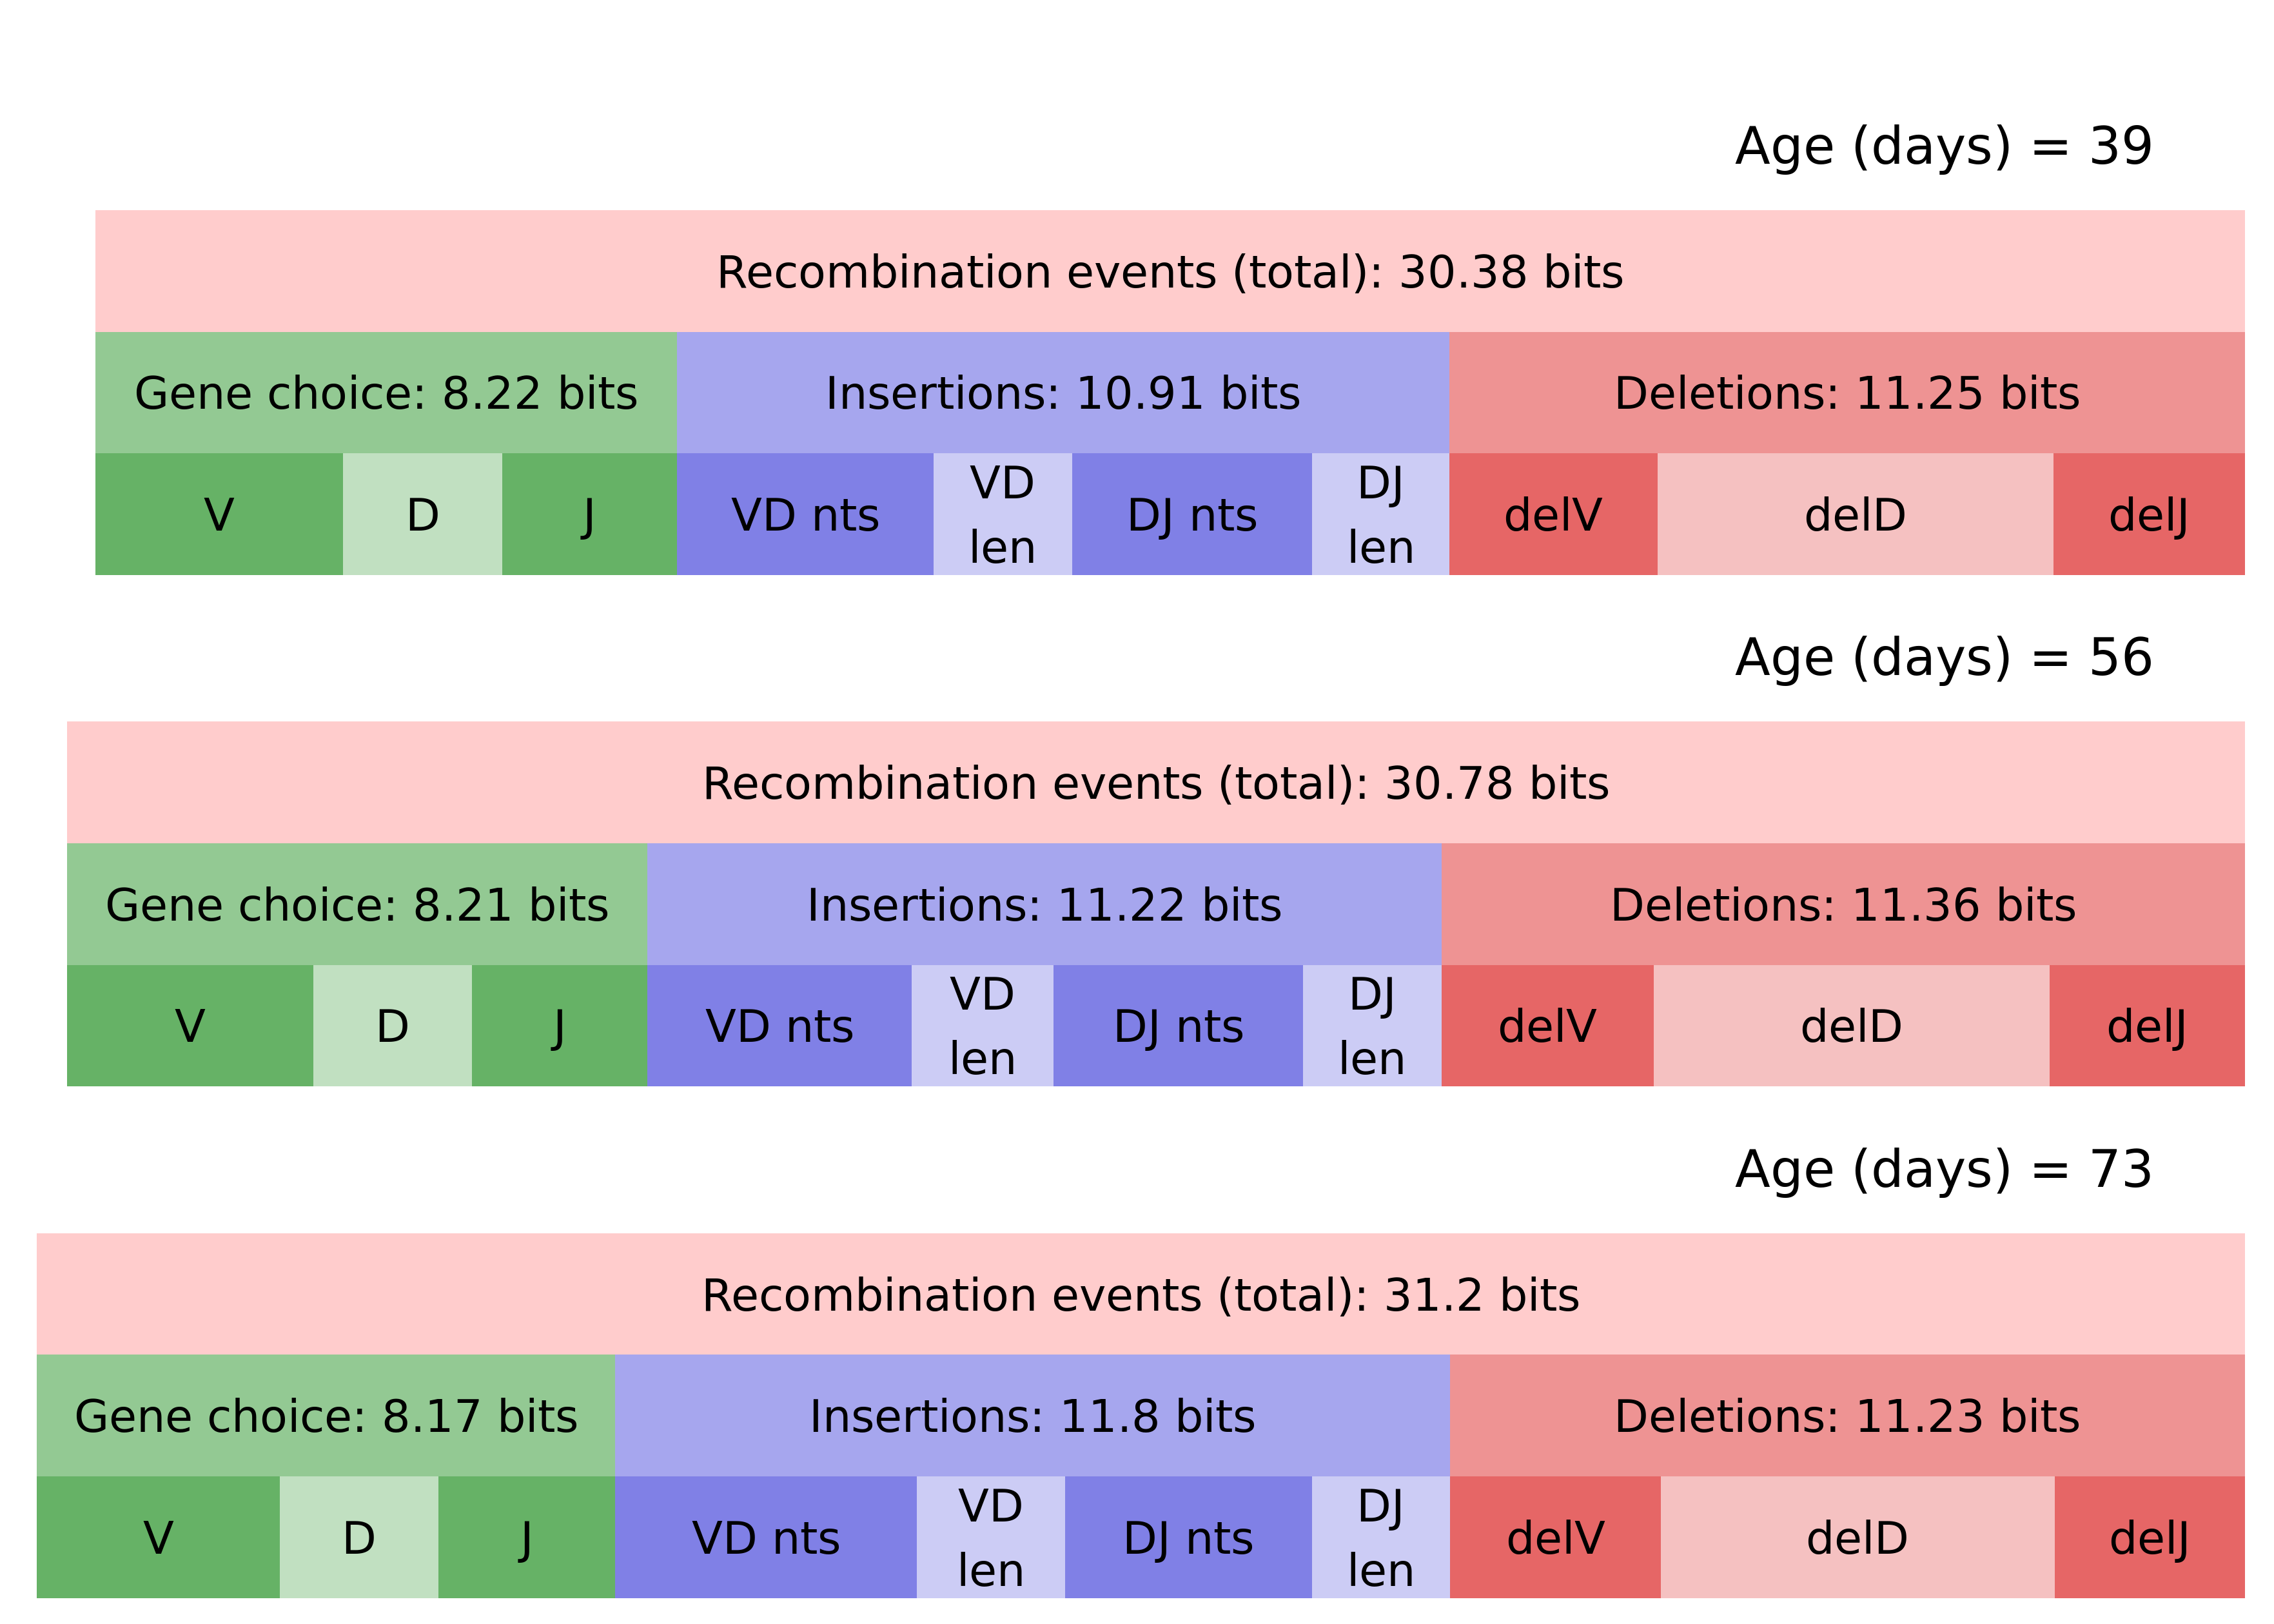
\includegraphics[height=0.95\slideheight]{../_Figures/png/ageing-igor-entropies}
\end{figure}
\end{frame}



\end{document}

